Les nombres de Mersenne sont les nombres qui s'expriment sous la forme :

\begin{center}
$M_{n} = 2^{n}-1, n\geq1$
\end{center}

A partir de cette séquence, on trouve la sous-suite des nombres premiers de Mersenne, composée comme son nom l'indique des nombres de Mersenne qui sont aussi premiers.\\
De par la simplicité de leur expression et la progression exponentielle de la suite, ces nombres battent régulièrement le record du plus grand nombre premier connu, le dernier en date étant $M_{82 589 933}$, un nombre constitué d'environ 25 millions de chiffres en base 10 découvert en décembre 2018.\\
Nous avons essayé de parcourir la suite des nombres de Mersenne pour trouver les termes premiers de deux façons différentes : via la recherche dans un fichier et via un test de primalité.

\subsection{Recherche des nombres premiers dans une liste}
Nous avons alors recherché les nombres premiers de Mersenne parmi une liste de 300 000 000 nombres premiers générée avec la méthode d'exponentiation modulaire décrite en première partie.
Avec cette méthode, le plus grand nombre de Mersenne trouvable est $M_{31}=2 147 483 647$.
Il a fallu environ deux heures pour trouver tous les nombres.

\subsection{Test de Lucas-Lehmer}
Le test de Lucas-Lehmer est un test de primalité spécifique aux nombres de Mersenne. Il fonctionne de la manière suivante :

Soit $s_{i}$ la suite définie par $s_{0}=4$ et $s_{i+1}=s_{i}^{2}-2$.
Pour $p>2$, $M_{p}$ est premier si et seulement si $s_{p-2} mod M_{p} = 0$.

Nous avons mesuré le temps nécessaire au test pour les nombres jusqu'à $M_{31}$ :
\begin{figure}[!h]
\begin{center}
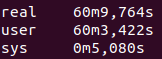
\includegraphics[scale=0.5]{images/benchmark_lucas.png}
\end{center}
\caption{Résultat du test de Lucas-Lehmer appliqué de $M_{3}$ à $M_{31}$}
\end{figure}

En outre, nous avons mesuré l'évolution du temps de calcul du test de primalité en fonction de l'indice dans la suite :
\begin{figure}[!h]
\begin{center}
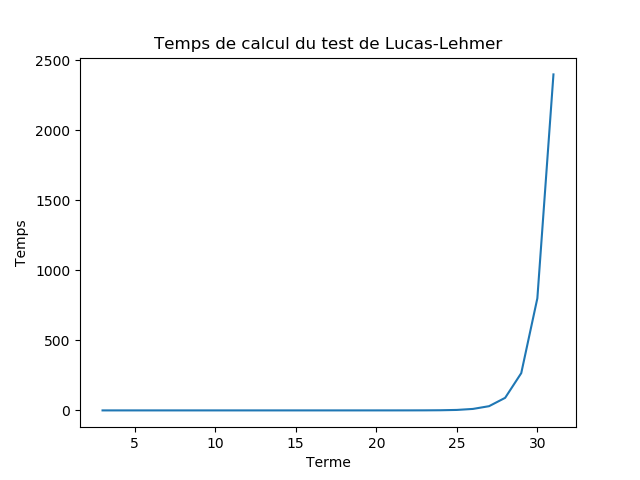
\includegraphics[scale=0.5]{images/evo_lucas.png}
\end{center}
\caption{Évolution du temps de calcul jusqu'à $M_{31}$}
\end{figure}

On observe que le temps de calcul augmente de façon exponentielle, ce qui était prévisible étant donné que le test est basé sur une suite définie par récurrence.\\

\subsection{Conclusion}
Si le test de Lucas-Lehmer est extrêmement rapide au début, il devient vite inefficace par rapport à une recherche dans une liste qui s'effectue en temps constant ; cependant l'utilisation d'un fichier crée un vrai problème de mémoire pour la recherche de grands nombres.
